\section{Approach}
\label{sec:approach}
In this section, 
we first introduce the length-controllable summarization problem and its basic models,
then introduce the length-aware attention mechanism, which attends the existing
transformer seq2seq models, and finally explain how to pretrain LAAM using 
a length-balanced dataset. 

\subsection{Preliminaries}
In length-controllable summarization, the model takes the source document 
$\mathbf{x} = (x_{0},x_{1},...,x_{m})$ and the desired length $l$ as input and the summary $\mathbf{y} = (y_{0},y_{1},..., y_{n})$ as output(i.e. $m>n$).
$x_i$ is the $i^{th}$ token in the input document and
$y_t$ is the $t^{th}$ token in the output summary.
$x_{m}$ and $y_{n}$ are $eos$ tokens.
%As the desired length $l$ is number of the tokens in summary except $eos$, $l=n+1$.
The goal is to estimate the conditional probability
$p(\mathbf{y}|\mathbf{x})$:
\begin{equation}
	p(\mathbf{y} | \mathbf{x}) \!=\! {\prod^T_{t} {p(y_{t} | y_{1}, y_{2},..., y_{t-1}, \mathbf{x},l})}
\end{equation}

Recent successful summarization models are based on transformer 
seq2seq models~\cite{attn17}, which will be the basis of our approach in
this work.  
In basic transformer seq2seq models, the encoder and decoder are both
multi-layered. The encoder output is $\mathbf{h}=\left\{h_0,h_1,...,h_m\right\}$,  
$\mathbf{h} \in \mathbb{R}^{m \times d}$,
and the output of the decoder's masked self-attention sub-layer 
is $\mathbf{z}=\left\{z_0,z_1,...,z_n\right\}$,
$\mathbf{z} \in \mathbb{R}^{n \times d}$.
The normal cross-attention layer is calculated as:
\begin{equation}
	\mathbf{A}=softmax(\textbf{z} \cdot \textbf{h}^T)
\end{equation}
where $\mathbf{A} \in R^{n\times m}$ are attention scores.
$A_{t}=\left\{a_{t,0}, a_{t,1},...,a_{t,m}\right\}$ denotes the attention scores. %between output token $y_t$ and all of the input tokens in $\mathbf{h}$.
$a_{t,i}$ is the attention score between $y_t$ and $x_i$.



\subsection{Length-aware Attention Mechanism (LAAM)}
\label{sec:model} 
In this work, we improve the transformer seq2seq models by renormalizing 
the cross-attention based on length.

The cross-attention of a token $y_t$ in decoder shows 
the alignment between this token and all of the input tokens in encoder.
$y_j$ is more likely to be summarized from tokens with a higher attention score in the encoder.
%The input tokens with higher attention scores have higher probability of summarizing $y_j$.
Thus, we propose {\bf a length-aware attention mechanism} to enlarge the attention of some tokens in $\textbf{x}$ based on length, which helps model to learn to choose which tokens to be summarized according to different desired lengths.
The length-aware attention mechanism is illustrated in \figref{fig:model_main}.
This mechanism is made up of two parts: {\em attention based on information selection} and 
{\em attention based on $eos$}.
 
\begin{figure}[th]
	\centering
	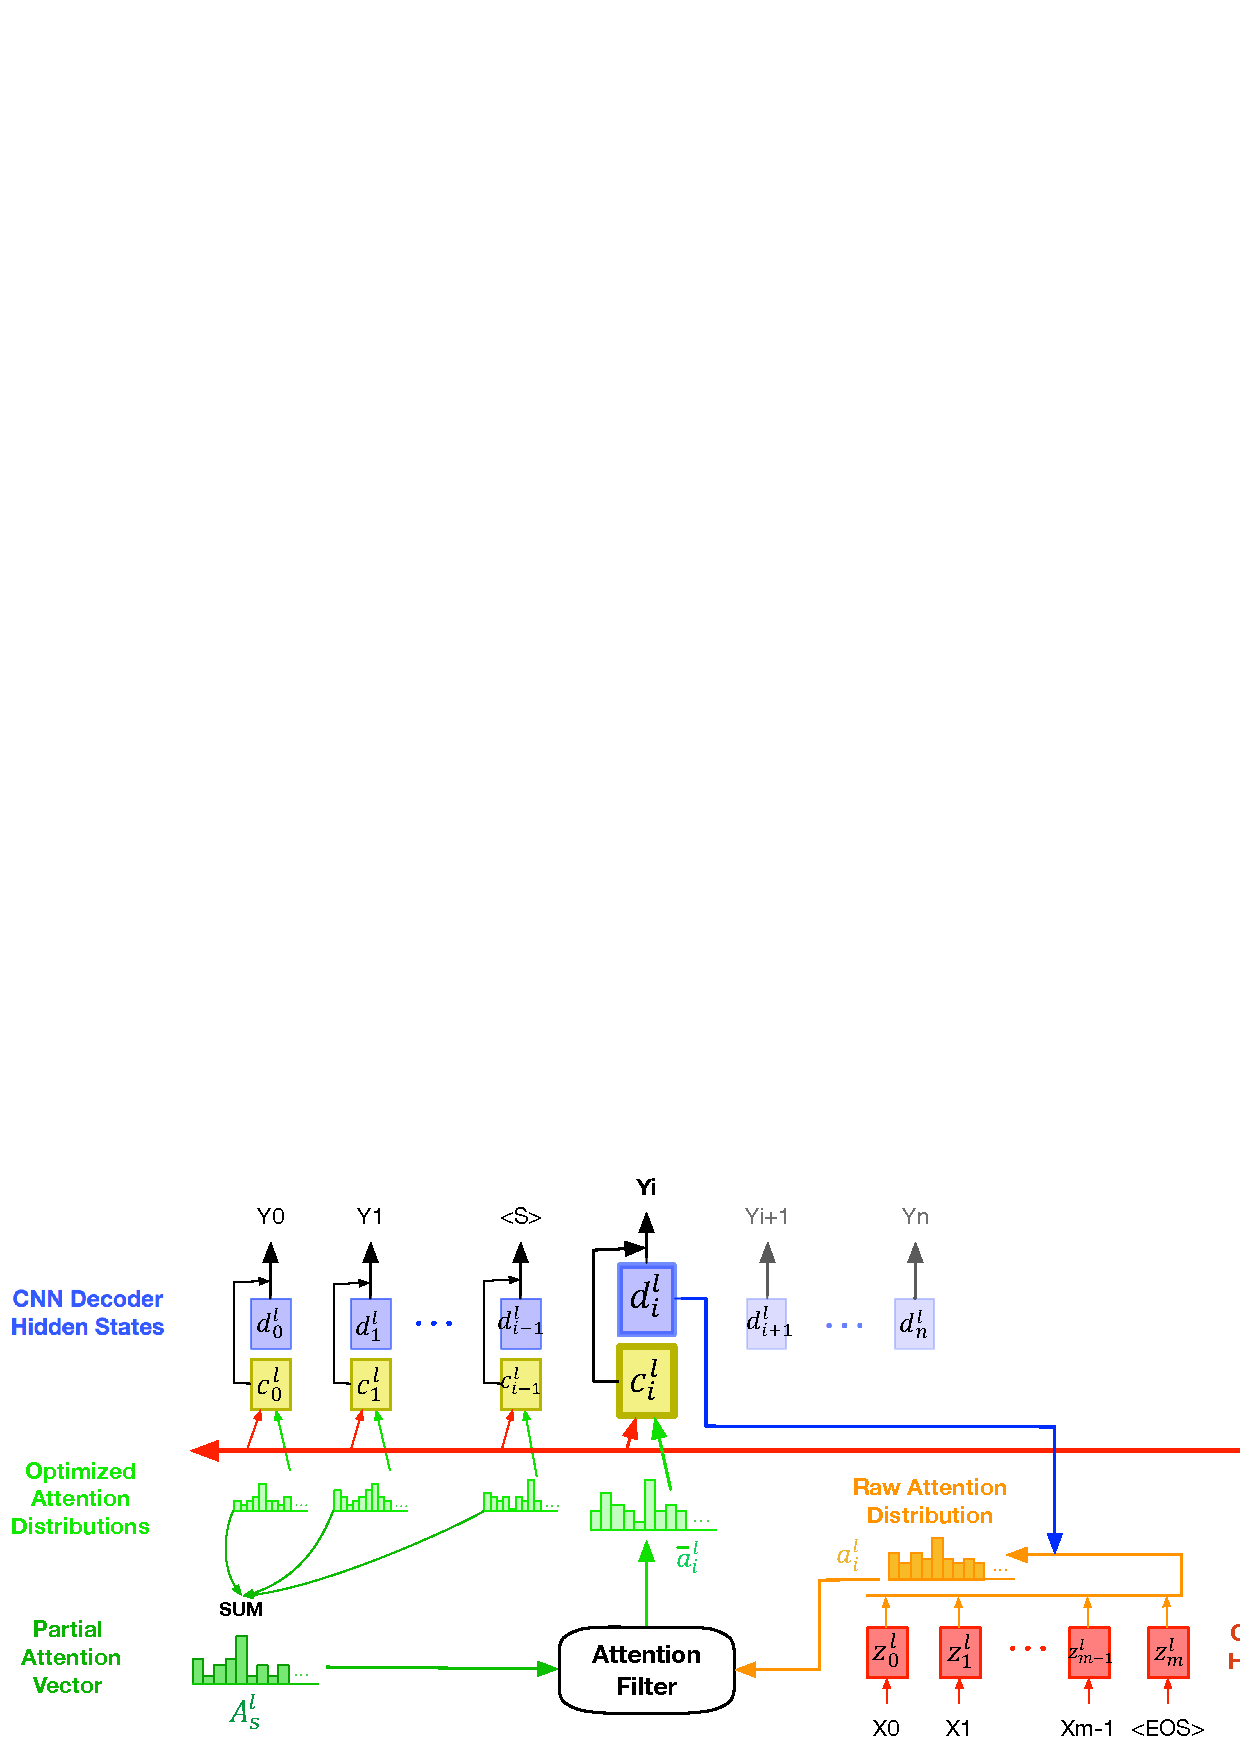
\includegraphics[width=1.0\linewidth]{model.pdf}
	\caption{Overview of LAAM on Transformer Seq2seq}
	\label{fig:model_main}
\end{figure}


\subsubsection{Attention based on information selection ($Attn_{is}$)}
In the decoding process,
we take the {\em remaining length} $l_t$
as additional input to re-normalize attention $A_{t}$ as follows:

 \begin{align}
        l_t &=		
		\begin{cases}			
			l+1-t, &\mbox{$0\leq t \leq l$}\\			
			1, &\mbox{otherwise}			
		\end{cases}		
%	\\
%	   L &=l+1
\end{align}
where $t$ is timestamp. 
$l+1$ is the number of tokens in the output with $eos$.

At each decoding step $t$, the decoder should plan its output $y_t$ based on the remaining number $l_t$ of tokens it will generate.
So we modify the $A_t$ by enlarging the attention of the top $l_t$ tokens with highest attention scores in it,
which makes decoder trend to output $y_t$ expressing the information of these enhanced tokens. 
In this way, the longer desired length $l$, the more source information should be selected for summarizing. 
The model ends the generation through the attenuation of selected information. 

To compute the $Attn_{is}$, we first use one-hot vector $\mathbf{p}=\left\{p_0,p_1,...,p_m\right\}$ to label the indices of the top $l_t$ tokens with highest attention scores in $A_t$ as $1$ and others as $0$, and then compute the length-aware attention as follows:
 \begin{equation}
 	a'_{t,i}=w_{t,i} \times a_{t,i} \\
\end{equation}
\begin{equation}\label{eq:w}
 	w_{t,i}=
 	\begin{cases}			
 		1, &\mbox{$p_i=0$}\\			
 		l_t, &\mbox{$p_i=1$}			
 	\end{cases}	
 \end{equation}
%where $w_{t,i}$ denotes the magnification of the $i$ token in source document at step $t$. \JQ{wo yun le}
where $w_{t,i}$ is the {\em weight for boosting the attention} between the $i^{th}$ token in source document and $t^{th}$ token in summary.
According to \eqnref{eq:w},  
the weigth for cross-attention decreases as the remaining length decreases,
resulting in a decrease in the gap between the enhanced tokens and other tokens. 
At a shorter remaining length, 
the model trends to output the general word to 
express the enhanced tokens and end the decoding.
%As the output token at a shorter remaining length
%should be summarized from the enhanced tokens and 
The general word means the model should evenly attend to
%take account into more information 
tokens related to the enhanced tokens.
This needs to decrease the gap between the enhanced token and other related tokens,
which is consistent with our design.
%The weight of the tokens with highest attention scores in $A_t$ is $l_t$,
We boost the attention score in $A_t$ by $l_t$
which makes the weights for the attention of the last token in output with different desired lengths the same by successively decreasing.
%We expect the model to learn the relation between the attention distribution of last output tokens and the generating $eos$.
We expect the model to learn to predict $eos$ based on the decreasing of weight for attention.

\subsubsection{Attention based on $\bf eos$ ($Attn_{eos}$)}
To enhance the ability of model to control length,
we modify the attention score of $eos$ at each decoding step.
As $eos$ in source document is represented as $y_n$, we calculate $Attn_{eos}$ as:
\begin{equation}
 	a'_{t,m}=(l+1-l_t) \times a_{t,m} \\
\end{equation}
The length-aware attention of $eos$ increases step by step, 
which demonstrates the probability of stopping decoding will increase
as the length of the output close to the desired length.


Finally, we re-normalize the modified attention scores $A'_t=\left\{a'_{t,0}, a'_{t,1},...,a'_{t,m}\right\}$ to get the context vector $\mathbf{c_t}$ and compute the probability distribution of predicted tokens via:
\begin{align}
	p(y_t|y_0,...,y_{t-1},\mathbf{x},l) &=softmax(W \mathbf{c}_{t-1}+b) \\
	\mathbf{c_t} &=\sum_{0}^{m} \tilde{a}_{t,i} h_i \\
	\tilde{a}_{t,i} &= \frac{a'_{t,i}}{\sum_{i=0}^{m}a'_{t,i}}
\end{align}
where $W$ and $b$ are trainable parameters.


\cut{%%%%%
We use $h^p_{i}$ to denote the encoder hidden state for $i$-th tokens.
We describe $l$ as the desired length.
The representation of $j$-th special token, $s^p_{j}$.
Then we aggregate the information through Convolutional Neural Network
as:
\begin{equation}
	S_j = CNN(h_{i}, S_{j-1})
\end{equation}
%The last hidden state $H^p_U$.
where $S_j$ is the encoder hidden state of the $j$-th tokens.
Similary, we can get the $l$-th tokens as following:
\begin{equation}
	\tilde{S}_l = \tanh(WS_l+W'l+b)
\end{equation}

where $v$ denote the randomly initialized context vector of encoder.
$W$ and $b$ are parameters.
At each decoding step $t$, 
$C_t$ is the weighted sum of encoder hidden states with cross-attention between encoder and decoder as weight. 
\begin{align}
	a_t &= \frac{\exp(\tilde{S}_lv_j)}{\sum_{0}^{l}{\exp(\tilde{S}_lv_j)}} \\
	C_t &= \sum_{t=0}{a_th_i}
\end{align}
}%%%%%

\subsection{LBD Creation for Pretraining LAAM}
\label{sec:lbd}
Neural-based abstractive summarization models
generate summaries whose length depends on the length distribution of training summaries.
As the summary lengths in different length ranges of a training dataset 
are always imbalanced,
we create a length-controllable dataset for each original dataset, which consists of the source documents and 
their extractive summaries within variant lengths. The lengths of summaries in LBD are evenly distributed in different ranges. 
Because the summaries of LBD are extractive, the model training on LBD can learn how to extract information with different input lengths.

Given an original abstractive summarization dataset $D_o$, we create training set $T_{l}$ and validation set $V_{l}$ of length-controllable dataset $D_l$ for $D_o$. 
$T_{o}$ and $V_{o}$ denote original training set and validation set respectively.
The number of the samples in $T_{o}$ is $N_{o}^t$.

To create $T_{l}$, 
we set the discrete bins $B=\left\{B_1, B_2,...,B_k\right\}$ to represent the ranges of summary length of $T_{l}$. 
$k$ is the number of the bins. 
$B_i=\left(minLen_i, maxLen_i\right)$ is the $i^{th}$ length range. 
For example, $B=\left\{(0,10],(10,30],...,(90, +\infty)\right\}$ and $B_0=(0,10]$. 
For each source document $src$ and its reference summary $ref$ in $T_{o}$,
%we produce length-controllable pairs (LCPs) consisting of $src$ and its the 
we produce length-controllable pairs (LCPs) consisting of $src$ and its the 
extractive summaries in different length ranges.
$ext_i$ is the extractive summary with length in $B_i$.
%which should be added into $S(B_i)$.
We apply a greedy approach,
where we add one sentence at a time incrementally to the $ext_i$, 
such that $ext_i$ has length within $B_i$ and has highest ROUGE-1 (R-1) recall with respect to $ref$.
Generally, the more training data, the greater the impact on the model.
To make $T_{l}$ effective,
the number of samples in $T_{l}$ should be close to $N_{o}^t$.
%$N(B_i)$ as the number of $S(B_i)$ is $\lceil N_{ot}/k \rceil$.
We add top $\lceil N_{o}^t/k \rceil$ extractive summaries (length $\in B_i$) 
with highest R-1 recall and their source documents to $S(B_i)$,
which makes the number of summaries in different length ranges balanced.
$S(B_i)$ is the subset of $T_{l}$, including LCPs with extractive summaries with length in $B_i$. 
The details are in \algoref{alg:data}.


\begin{algorithm}[th!]
	\caption{Length-controllable Training Data Creation}
	\label{alg:data}
	\scriptsize
	\textbf{Input}: the training set $T_{o}$  of original dataset $D_o$ \\
	%\textbf{Parameter}: Optional list of parameters\\
	\textbf{Output}:  the training set $T_{l}$ of length-controllable dataset $D_l$ \\
	\begin{algorithmic}[1] %[1] enables line numbers
		\STATE $rec()$ computes the R-1 recall score between two texts.
		\STATE $len()$ computes the length of token sequence.
		\FOR {\textbf{each} training pair ($src$, $ref$) $\in T_{o}$}
		%\STATE ($src$, $ref$) is the $j^{th}$ training pair of $D_{ot}$.
		\STATE $src=\left\{s_0, s_1,...\right\}$, where $s_t$ is the $t^{th}$ sentence in $src$.
		\FOR {$i=0 \rightarrow k$}
		%\STATE $ext_i$ is the extractive summary with length in range $B_i$.
		\STATE $ext_i \leftarrow \emptyset$
		%\WHILE{select the $s_{sel}$ with best $rec(ext_i\cup s_{sel}, ref)$ from $\left\{s|s \in src \cap len(ext_i \cup s) \leq maxL_i \right\}$}
		\WHILE{$S=\left\{s|s \in src \cap len(ext_i \cup s) \leq maxL_i \right\}$}
	    \STATE Select the $s_{sel}$ with best $rec(ext_i\cup s_{sel}, ref)$ from $S$.
		%\WHILE{exist $s$ of $src$ and $len(ext_i \cup s) \leq maxLen_i$}
		\IF{$rec(ext_i\cup s_{sel}, ref) \textgreater rec(ext_i, ref)$}
		\STATE $ext_i \leftarrow s_{sel}$; $src \leftarrow src-s_{sel}$
		\ELSE 
		\STATE break
		\ENDIF
		\ENDWHILE
		\IF{$len(ext_i) \textgreater minL_i$}
		\STATE Add $(src, ext_i, rec(ext_i,ref))$ to $S(B_i)$.
		\ENDIF
		\ENDFOR
		\ENDFOR
		\STATE $S(B_i) \leftarrow$ the top $\lceil N_{o}^{t}/k \rceil$ samples from $S(B_i)$ sorted by $rec(ext_i,ref)$
		\STATE $T_{l} \leftarrow S(B_1) \cup S(B_2)\cup \cdots \cup S(B_k)$
		\RETURN $T_{l}$
	\end{algorithmic}
\end{algorithm}


For $V_{l}$, 
we select a sentence at a time until we get the best combination of sentences from $src$ as extractive summary that maximizes the R-1 F1 
%\KZ{explain why F1 and not recall any more?} 
with respect to $ref$. 
%In this approach, R-1 recall computes the percentage of the tokens in the reference summary are also present in extractive summary, and R-1 F1 will  
Given an original source document and reference summary pair, 
%n this approach, 
R-1 recall compute the similarity between extracted sentences and reference without considering the length of extracted sentences.
This meets our requirements for creating $T_{l}$, that is, we can extract multiple summaries within different length ranges for one document.
%These extractive summaries are most similar to reference summaries
%Different from creating $T_{l}$, 
To evaluate the model at training,
each document in $V_l$ only needs one extractive summary.
R-1 F1 considers difference between the lengths of compared summaries, 
which can select a extractive summary most similar to reference in length and content.
%R-1 F1 
%Thus, we apply R-1 F1 to get extractive summary, which makes extractive summary most similar to its reference summary on length and content.
%Length bins are chosen so that they each contain roughly an equal number of training documents. 


\cut{%%%%%
\begin{algorithm}[th!]
\caption{Length-controllable Training Data Creation}
\label{alg:data}
\small
\textbf{Input}: the training set $D_{ot}$  of original dataset $D_o$ \\
%\textbf{Parameter}: Optional list of parameters\\
\textbf{Output}:  the training set $D_{lt}$ of length-controllable dataset $D_l$ \\
\begin{algorithmic}[1] %[1] enables line numbers
\STATE Let $N_{ot}$ be the number of samples in $D_{ot}$.
\STATE Set discrete bins $B=\left\{B_1, B_2,...,B_k\right\}$ to represent the ranges of summary length of $D_{lt}$. $B_i=\left(minL_i, maxL_i\right)$. For example, $B=\left\{(0,10],(10,30],...,(90, +\infty]\right\}$, $B_0=(0,10]$. 
\STATE $k$ is the number of bins. 
\STATE $N(B_i)$ denotes the number of samples with summary length in range $B_i$. 
\STATE $S(B_i)$ contains the samples in $D_{lt}$ with summary length in range $B_i$.
\STATE $N(B_i) \leftarrow \lceil N_{ot}/k \rceil$.
\STATE $S(B_i) \leftarrow \emptyset$.
%\STATE $rec()$ and $f()$ computes the ROUGE-1 recall and F1 score between two texts.
\STATE $rec()$ computes the ROUGE-1 recall score between two texts.
\STATE $len()$ computes the length of token sequence.
\FOR {$j=0 \rightarrow N_{ot}$}
\STATE $P_j$ is the $j^{th}$ training pair in $D_{ot}$, which consists of source document $src$ and reference summary $ref$.
\STATE $src=\left\{s_0, s_1,...\right\}$ consisting of multiple sentences. $s_t$ is the $t^{th}$ sentence in $src$.
\FOR {$i=0 \rightarrow k$}
\STATE $ext_i$ is the extractive summary with length in range $B_i$.
\STATE $ext_i \leftarrow \emptyset$
\WHILE{Select the $s_{sel}$ with best $rec(ext_i\cup s_{sel}, ref)$ from $\left\{s|s \in src \cap len(ext_i \cup s) \leq maxLen_i \right\}$}
%\STATE $Set=\left\{s|s \in src \cap len(ext_i \cup s) \leq maxLen_i \right\}$
%\WHILE{$Set$ is not empty}
%\STATE $Sel$ is the set of sentences $s$ in $Set$ with highest $rec(ext_i\cup s_{sel}, ref)$
%\STATE Select $s_{sel}$ from $Sel$ with highest$f(ext_i\cup s_{sel}, ref)$
\IF{$rec(ext_i\cup s_{sel}, ref) \textgreater rec(ext_i, ref)$}
\STATE $ext_i \leftarrow s_{sel}$
\STATE $src \leftarrow src-s_{sel}$
\ELSE
\STATE break
\ENDIF
\ENDWHILE
\IF{$len(ext_i) \textgreater minLen_i$}
\STATE $S(B_i) \leftarrow (src, ext_i, len(ext_i), rec(ext_i,ref))$
\ENDIF
\ENDFOR
\ENDFOR
\STATE $S(B_i) \leftarrow$ the top $N(B_i)$ samples from $S(B_i)$ sorted by $rec(ext_i,ref)$
\STATE $D_{lt} \leftarrow S(B_1) \cup S(B_2)\cup \cdots \cup S(B_k)$
\STATE return $D_{lt}$
\end{algorithmic}
\end{algorithm}

\begin{algorithm}[th!]
	\caption{Length-controllable Validation Data Creation}
	\label{alg:valid}
	\small
	\textbf{Input}: the validation set $D_{ov}$  of original dataset $D_o$ \\
	%\textbf{Parameter}: Optional list of parameters\\
	\textbf{Output}:  the validation set $D_{lv}$ of length-controllable dataset $D_l$ \\
	\begin{algorithmic}[1] %[1] enables line numbers
		\STATE Let $N_{ov}$ be the number of samples in $D_{ov}$.
		\STATE $f()$ computes the ROUGE-1 F1 score between two texts.
		\STATE $len()$ computes the length of token sequence.
		\FOR {$j=0 \rightarrow N_{ov}$}
		\STATE $P_j$ is the $j^{th}$ validation pair in $D_{ov}$, which consists of source document $src$ and reference summary $ref$.
		\STATE $src=\left\{s_0, s_1,...\right\}$ consisting of multiple sentences. $s_t$ is the $t^{th}$ sentence in $src$.
		\STATE Extractive summary $ext_i \leftarrow \emptyset$
		\WHILE{$f(ext_i\cup s_{sel}, ref) \textgreater f(ext_i, ref)$}
		\STATE $ext_i \leftarrow s_{sel}$
		\STATE $src \leftarrow src-s_{sel}$
		\ENDWHILE
		\STATE Add sample $(src, ext_i, len(ext_i))$ into $D_{lv}$
		\ENDFOR
		\STATE return $D_{lv}$
	\end{algorithmic}
\end{algorithm}
}%%%%%


As the summaries in LBD
are extractive summaries with proper length distribution,
we first train LAAM on LBD
as pretrained model to learn to select the information from source document to be summarized according to length constraint.
Then we fine-tune the pretrained LAAM ({\bf PtLAAM}) on original training data.
In this way, on the basis of selecting information from source document, 
the model further learns to paraphrase the selected information into abstractive summaries with desired length.

